% type:ignore

\chapter{Resultados Computacionais}

% \section{Modelos Matemáticos}
% Embora três modelos matemáticos tenham sido propostos — a formulação independente e as formulações comportamentais —, ao resolver as instâncias decidiu-se inicialmente testar os modelos sem as restrições de fulfillment nem as restrições de skiplagging. Em seguida, cada modelo foi testado separadamente com cada grupo de restrições. Por fim, ambos os modelos foram avaliados considerando os dois conjuntos de restrições simultaneamente. Essa abordagem foi adotada para observar como a solução evoluía ou se comportava ao incluir cada tipo de restrição no modelo. Dito isso, a seguir são apresentados os modelos com suas respectivas descrições.
% \vspace{0.5cm}

% \begin{small}
% 	\begin{longtable}{p{5.4cm} p{10.4cm}}
% 		\hline
% 		\textbf{Tipo de Modelo}            & \textbf{Descrição}                                                                                                                       \\ \hline
% 		BaseModel                          & Modelo base independente sem as restrições de Fulfillments nem as restrições de Skiplagging.                                             \\ \hline
% 		BaseModelFulfillments              & Modelo base independente com as restrições de Fulfillments.                                                                              \\ \hline
% 		BaseModelSkiplagging               & Modelo base independente com as restrições de Skiplagging.                                                                               \\ \hline
% 		BaseModelFull                      & Modelo independente completo com os dois conjuntos de restrições.                                                                        \\ \hline
% 		HierarBehavioralModel              & Modelo base comportamental com ajuste de demanda do tipo hierarquia, sem as restrições de Fulfillments nem as restrições de Skiplagging. \\ \hline
% 		HierarBehavioralModelFulfillments  & Modelo base comportamental com ajuste de demanda do tipo hierarquia, com as restrições de Fulfillments.                                  \\ \hline
% 		HierarBehavioralModelSkiplagging   & Modelo base comportamental com ajuste de demanda do tipo hierarquia, com as restrições de Skiplagging.                                   \\ \hline
% 		HierarBehavioralModelFull          & Modelo comportamental completo com ajuste de demanda do tipo hierarquia, com os dois conjuntos de restrições.                            \\ \hline
% 		PercentBehavioralModel             & Modelo base comportamental com ajuste de demanda do tipo proporção, sem as restrições de Fulfillments nem as restrições de Skiplagging.  \\ \hline
% 		PercentBehavioralModelFulfillments & Modelo base comportamental com ajuste de demanda do tipo proporção, com as restrições de Fulfillments.                                   \\ \hline
% 		PercentBehavioralModelSkiplagging  & Modelo base comportamental com ajuste de demanda do tipo proporção, com as restrições de Skiplagging.                                    \\ \hline
% 		PercentBehavioralModelFull         & Modelo comportamental completo com ajuste de demanda do tipo proporção, com os dois conjuntos de restrições.                             \\ \hline
% 		\caption{Descrição dos modelos matemáticos propostos}
% 		\label{tab:modelos}
% 	\end{longtable}
% \end{small}


% \section{Instâncias}

% Para verificar as características dos modelos propostos, foram utilizadas 10 instâncias reais fornecidas pela empresa canadense Expetrio. As características de cada uma dessas instâncias estão apresentadas na Tabela \ref{tab:instancias}.

% \begin{table}[H]
% 	\centering
% 	\begin{tabular}{ccccccc}
% 		\toprule
% 		\textbf{Instância}                                                  &
% 		\textbf{\begin{tabular}[c]{@{}c@{}}Nome \\ Trem\end{tabular}}       &
% 		\textbf{\begin{tabular}[c]{@{}c@{}}Capacidade \\ Trem\end{tabular}} &
% 		\textbf{Data Partida}                                               &
% 		\textbf{\# Trechos}                                                 &
% 		\textbf{\# Períodos}                                                &
% 		\textbf{\# Classes}                                                                                          \\
% 		\midrule
% 		Inst1                                                          & 68 & 561 & 2023-11-21 & 256 & 120 & 15 \\
% 		Inst2                                                          & 13 & 637 & 2023-11-26 & 252 & 146 & 15 \\
% 		Inst3                                                          & 71 & 563 & 2023-10-13 & 250 & 105 & 16 \\
% 		Inst4                                                          & 71 & 561 & 2023-11-21 & 241 & 124 & 15 \\\midrule
% 		Inst5                                                          & 8  & 561 & 2022-12-04 & 152 & 116 & 17 \\
% 		Inst6                                                          & 40 & 565 & 2023-11-21 & 149 & 68  & 16 \\
% 		Inst7                                                          & 74 & 491 & 2023-07-25 & 136 & 70  & 16 \\\midrule
% 		Inst8                                                          & 72 & 493 & 2023-10-25 & 100 & 85  & 16 \\
% 		Inst9                                                          & 45 & 563 & 2023-03-16 & 90  & 73  & 16 \\
% 		Inst10                                                         & 15 & 493 & 2023-08-07 & 50  & 60  & 12 \\
% 		\bottomrule
% 	\end{tabular}
% 	\caption{Resumo das instâncias utilizadas no experimento}
% 	\label{tab:instancias}
% \end{table}

% A coluna "\# Trechos" \, representa a quantidade de trechos que a viagem do trem possui em cada instância. A coluna "\# Períodos" \, indica a quantidade de períodos considerados na programação desse trajeto dentro do seu horizonte de reserva. Por fim, a coluna "\# Classes" \, mostra o número máximo de classes disponíveis para cada viagem de cada trem; Observe que, para cada trecho, podem estar disponíveis todas as classes indicadas na coluna correspondente ou uma quantidade menor.

% Por outro lado, afirmamos que as instâncias compreendidas entre a Instância1 e a Instância4 são classificadas como grandes, as instâncias entre a Instância5 e a Instância7 como médias, e as demais como pequenas.

\section{Experimentos Computacionais}
Para resolver as instâncias utilizando os modelos matemáticos propostos, foi empregado um computador da marca Dell, modelo Precision 3660, equipado com o sistema operacional Windows 11 Pro de 64 bits, processador 13th Gen Intel(R) Core(TM) i7-13700 2.10 GHz baseado em arquitetura x64, e memória RAM de 16GB. Além disso, utilizou-se o Python como linguagem de programação na versão 3.10.14, e o solver Gurobi na versão 11.0.3.

Em primeiro lugar, apresentam-se os resultados de cada instância após serem resolvidas por meio de cada um dos modelos propostos. Essa organização busca evidenciar de forma clara e comparativa o desempenho dos modelos em diferentes cenários, destacando as principais diferenças e similaridades nas soluções obtidas para cada instância.

Observe que a primeira coluna indica o nome do modelo utilizado. A segunda coluna, "\textit{T. Criação Modelo (seg.)}", exibe o tempo, em segundos, que o solver levou para construir o modelo. A terceira coluna, "\textit{T. Solução (seg.)}", mostra o tempo necessário para que o solver resolvesse o modelo. A sétima coluna, "\textit{Z Relaxado}", apresenta a relaxação linear do problema no nó raiz. Já a oitava coluna, "\textit{Z\*}", indica o valor ótimo da função objetivo (máximo lucro encontrado). Por fim, a nona coluna, "\textit{$ \Delta Z (\%)$}", mostra a diferença percentual entre a solução relaxada e a solução ótima.

\begin{table}[H]
    \centering
    \resizebox{\textwidth}{!}{%
        \begin{tabular}{lccccccccc}
            \hline
            \textbf{Modelo} &
            \textbf{\begin{tabular}[c]{@{}c@{}}T. Criação \\ Modelo (seg.)\end{tabular}} &
            \textbf{\begin{tabular}[c]{@{}c@{}}T. Solução \\ (seg.)\end{tabular}} &
            \textbf{\begin{tabular}[c]{@{}c@{}}N° Nós \\ Explorados\end{tabular}} &
            \textbf{\begin{tabular}[c]{@{}c@{}}N° \\ Iterações\end{tabular}} &
            \textbf{\begin{tabular}[c]{@{}c@{}}N° \\ Soluções\end{tabular}} &
            \textbf{\begin{tabular}[c]{@{}c@{}}Z \\ Relaxado\end{tabular}} &
            \textbf{Z*} &
            \textbf{\begin{tabular}[c]{@{}c@{}}$\Delta$ Z \\ (\%)\end{tabular}} \\ \hline
            BaseModel & 2,30 & 0,07 & 1 & 0 & 1 & 170.485 & 170.485 & 0,00 \\ 
            BaseModelFulfillments & 3,97 & 0,07 & 1 & 0 & 1 & 170.485 & 170.485 & 0,00 \\ 
            BaseModelSkiplagging & 6,06 & 0,06 & 1 & 0 & 1 & 133.237 & 133.237 & 0,00 \\ 
            BaseModelFull & 6,43 & 0,05 & 1 & 0 & 1 & 51.410 & 51.410 & 0,00 \\ 
            HierarBehavioralModel & 3,17 & 0,07 & 1 & 0 & 1 & 170.455 & 170.455 & 0,00 \\ 
            HierarBehavioralModelFulfillments & 4,87 & 0,08 & 1 & 0 & 1 & 170.455 & 170.455 & 0,00 \\ 
            HierarBehavioralModelSkiplagging & 7,09 & 0,08 & 1 & 2 & 2 & 132.928 & 132.928 & 0,00 \\ 
            HierarBehavioralModelFull & 7,48 & 0,05 & 1 & 0 & 1 & 51.336 & 51.336 & 0,00 \\ 
            PercentBehavioralModel & 3,14 & 0,07 & 1 & 0 & 1 & 166.345 & 166.345 & 0,00 \\ 
            PercentBehavioralModelFulfillments & 4,90 & 0,08 & 1 & 0 & 1 & 170.455 & 170.455 & 0,00 \\ 
            PercentBehavioralModelSkiplagging & 7,07 & 0,06 & 1 & 2 & 2 & 132.928 & 132.928 & 0,00 \\ 
            PercentBehavioralModelFull & 7,47 & 0,05 & 1 & 0 & 1 & 51.336 & 51.336 & 0,00 \\ \hline
        \end{tabular}%
    }
    \caption{Resultados para a Instância1}
    \label{tab:resultado_instancia1}
\end{table}

\begin{table}[H]
    \centering
    \resizebox{\textwidth}{!}{%
        \begin{tabular}{lccccccccc}
            \hline
            \textbf{Modelo} &
            \textbf{\begin{tabular}[c]{@{}c@{}}T. Criação \\ Modelo (seg.)\end{tabular}} &
            \textbf{\begin{tabular}[c]{@{}c@{}}T. Solução \\(seg.)\end{tabular}} &
            \textbf{\begin{tabular}[c]{@{}c@{}}N° Nós \\Explorado\end{tabular}} &
            \textbf{\begin{tabular}[c]{@{}c@{}}N° \\Iterações\end{tabular}} &
            \textbf{\begin{tabular}[c]{@{}c@{}}N° \\Soluções\end{tabular}} &
            \textbf{\begin{tabular}[c]{@{}c@{}}Z \\Relaxado\end{tabular}} &
            \textbf{Z*} &
            \textbf{\begin{tabular}[c]{@{}c@{}}$\Delta$ Z \\(\%)\end{tabular}} \\ \hline
            BaseModel & 2,90 & 0,08 & 1 & 0 & 1 & 314.883,03 & 314.883,03 & 0,00 \\ 
            BaseModelFulfillments & 5,22 & 0,08 & 1 & 0 & 1 & 314.883,03 & 314.883,03 & 0,00 \\ 
            BaseModelSkiplagging & 7,47 & 0,07 & 1 & 0 & 1 & 303.634,13 & 303.634,13 & 0,00 \\ 
            BaseModelFull & 8,00 & 0,07 & 1 & 0 & 1 & 203.208,98 & 203.208,98 & 0,00 \\ 
            HierarBehavioralModel & 3,98 & 0,07 & 1 & 0 & 1 & 314.599,53 & 314.599,53 & 0,00 \\ 
            HierarBehavioralModelFulfillments & 6,38 & 0,10 & 1 & 0 & 3 & 314.599,53 & 314.599,53 & 0,00 \\ 
            HierarBehavioralModelSkiplagging & 8,58 & 0,06 & 1 & 0 & 1 & 303.375,63 & 303.375,63 & 0,00 \\ 
            HierarBehavioralModelFull & 9,11 & 0,07 & 1 & 0 & 1 & 203.276,98 & 203.276,98 & 0,00 \\ 
            PercentBehavioralModel & 3,98 & 0,07 & 1 & 0 & 1 & 313.547,03 & 313.547,03 & 0,00 \\ 
            PercentBehavioralModelFulfillments & 6,35 & 0,10 & 1 & 0 & 3 & 314.599,53 & 314.599,53 & 0,00 \\ 
            PercentBehavioralModelSkiplagging & 8,62 & 0,06 & 1 & 0 & 1 & 303.375,63 & 303.375,63 & 0,00 \\ 
            PercentBehavioralModelFull & 9,20 & 0,08 & 1 & 0 & 1 & 203.276,98 & 203.276,98 & 0,00 \\ \hline
        \end{tabular}%
    }
    \caption{Resultados para a Instância2}
    \label{tab:resultado_instancia2}
\end{table}


\begin{table}[H]
    \centering
    \resizebox{\textwidth}{!}{%
        \begin{tabular}{lccccccccc}
            \hline
            \textbf{Modelo} &
            \textbf{\begin{tabular}[c]{@{}c@{}}T. Criação \\ Modelo (seg.)\end{tabular}} &
            \textbf{\begin{tabular}[c]{@{}c@{}}T. Solução \\(seg.)\end{tabular}} &
            \textbf{\begin{tabular}[c]{@{}c@{}}N° Nós \\Explorado\end{tabular}} &
            \textbf{\begin{tabular}[c]{@{}c@{}}N° \\Iterações\end{tabular}} &
            \textbf{\begin{tabular}[c]{@{}c@{}}N° \\Soluções\end{tabular}} &
            \textbf{\begin{tabular}[c]{@{}c@{}}Z \\Relaxado\end{tabular}} &
            \textbf{Z*} &
            \textbf{\begin{tabular}[c]{@{}c@{}}$\Delta$ Z \\(\%)\end{tabular}} \\ \hline
            BaseModel & 2,25 & 0,05 & 1 & 33 & 2 & 140.788,61 & 140.788,61 & 0,00 \\ 
            BaseModelFulfillments & 3,75 & 0,08 & 1 & 377 & 2 & 140.788,61 & 140.788,61 & 0,00 \\ 
            BaseModelSkiplagging & 18,62 & 0,07 & 1 & 25 & 2 & 95.625,49 & 95.625,49 & 0,00 \\ 
            BaseModelFull & 19,15 & 0,05 & 1 & 0 & 1 & 37.214,03 & 37.214,03 & 0,00 \\ 
            \textbf{HierarBehavioralModel} &\textbf{3,01}&\textbf{0,08}& \textbf{1} & \textbf{97}&\textbf{6} & \textbf{140.179,10} & \textbf{140.167,27}& \textbf{0,01} \\ 
            \textbf{HierarBehavioralModelFulfillments} & \textbf{4,67} &\textbf{0,12} &\textbf{1} & \textbf{571}& \textbf{10} & \textbf{140.086,16}& \textbf{140.077,33} &\textbf{0,01} \\ 
            HierarBehavioralModelSkiplagging & 19,87 & 0,06 & 1 & 55 & 3 & 95.101,49 & 95.101,49 & 0,00 \\ 
            HierarBehavioralModelFull & 20,08 & 0,05 & 1 & 4 & 4 & 37.183,03 & 37.183,03 & 0,00 \\ 
            PercentBehavioralModel & 3,02 & 0,05 & 1 & 35 & 2 & 136.487,26 & 136.487,26 & 0,00 \\ 
            \textbf{PercentBehavioralModelFulfillments} & \textbf{4,67} & \textbf{0,12} & \textbf{1} &\textbf{571} &\textbf{10} & \textbf{140.086,16} &\textbf{140.077,33 }&\textbf{0,01} \\ 
            PercentBehavioralModelSkiplagging & 20,09 & 0,05 & 1 & 55 & 3 & 95.101,49 & 95.101,49 & 0,00 \\ 
            PercentBehavioralModelFull & 20,43 & 0,05 & 1 & 4 & 4 & 37.183,03 & 37.183,03 & 0,00 \\ \hline
        \end{tabular}%
    }
    \caption{Resultados para a Instância3}
    \label{tab:resultado_instancia3}
\end{table}


\begin{table}[H]
    \centering
    \resizebox{\textwidth}{!}{%
        \begin{tabular}{lccccccccc}
            \hline
            \textbf{Modelo} &
            \textbf{\begin{tabular}[c]{@{}c@{}}T. Criação \\ Modelo (seg.)\end{tabular}} &
            \textbf{\begin{tabular}[c]{@{}c@{}}T. Solução \\(seg.)\end{tabular}} &
            \textbf{\begin{tabular}[c]{@{}c@{}}N° Nós \\Explorado\end{tabular}} &
            \textbf{\begin{tabular}[c]{@{}c@{}}N° \\Iterações\end{tabular}} &
            \textbf{\begin{tabular}[c]{@{}c@{}}N° \\Soluções\end{tabular}} &
            \textbf{\begin{tabular}[c]{@{}c@{}}Z \\Relaxado\end{tabular}} &
            \textbf{Z*} &
            \textbf{\begin{tabular}[c]{@{}c@{}}$\Delta$ Z \\(\%)\end{tabular}} \\ \hline
            BaseModel & 2,20 & 0,05 & 1 & 0 & 1 & 166.118,29 & 166.118,29 & 0,00 \\
            BaseModelFulfillments & 3,70 & 0,08 & 1 & 0 & 1 & 166.118,29 & 166.118,29 & 0,00 \\
            BaseModelSkiplagging & 4,65 & 0,07 & 1 & 0 & 1 & 130.810,41 & 130.810,41 & 0,00 \\
            BaseModelFull & 4,95 & 0,04 & 1 & 0 & 1 & 40.602,31 & 40.602,31 & 0,00 \\
            HierarBehavioralModel & 3,02 & 0,05 & 1 & 0 & 1 & 165.869,29 & 165.869,29 & 0,00 \\
            HierarBehavioralModelFulfillments & 4,48 & 0,07 & 1 & 0 & 1 & 165.869,29 & 165.869,29 & 0,00 \\
            HierarBehavioralModelSkiplagging & 5,50 & 0,05 & 1 & 0 & 2 & 129.740,41 & 129.740,41 & 0,00 \\
            HierarBehavioralModelFull & 5,84 & 0,04 & 1 & 0 & 1 & 40.718,31 & 40.718,31 & 0,00 \\
            PercentBehavioralModel & 3,07 & 0,05 & 1 & 0 & 1 & 162.681,09 & 162.681,09 & 0,00 \\
            PercentBehavioralModelFulfillments & 4,52 & 0,08 & 1 & 0 & 1 & 165.869,29 & 165.869,29 & 0,00 \\
            PercentBehavioralModelSkiplagging & 5,47 & 0,07 & 1 & 0 & 2 & 129.740,41 & 129.740,41 & 0,00 \\
            PercentBehavioralModelFull & 5,73 & 0,05 & 1 & 0 & 1 & 40.718,31 & 40.718,31 & 0,00 \\ \hline
        \end{tabular}%
    }
    \caption{Resultados para a Instância4}
    \label{tab:resultado_instancia4}
\end{table}


\begin{table}[H]
    \centering
    \resizebox{\textwidth}{!}{%
        \begin{tabular}{lccccccccc}
            \hline
            \textbf{Modelo} &
            \textbf{\begin{tabular}[c]{@{}c@{}}T. Criação \\ Modelo (seg.)\end{tabular}} &
            \textbf{\begin{tabular}[c]{@{}c@{}}T. Solução \\(seg.)\end{tabular}} &
            \textbf{\begin{tabular}[c]{@{}c@{}}N° Nós \\Explorado\end{tabular}} &
            \textbf{\begin{tabular}[c]{@{}c@{}}N° \\Iterações\end{tabular}} &
            \textbf{\begin{tabular}[c]{@{}c@{}}N° \\Soluções\end{tabular}} &
            \textbf{\begin{tabular}[c]{@{}c@{}}Z \\Relaxado\end{tabular}} &
            \textbf{Z*} &
            \textbf{\begin{tabular}[c]{@{}c@{}}$\Delta$ Z \\(\%)\end{tabular}} \\ \hline
            BaseModel & 2,20 & 0,05 & 1 & 29  & 3 & 127.371,39 & 127.371,39 & 0,00 \\
            BaseModelFulfillments & 3,07 & 0,07 & 1 & 143 & 4 & 127.371,39 & 127.371,39 & 0,00 \\
            BaseModelSkiplagging & 3,05 & 0,07 & 1 & 0   & 1 & 95.816,84  & 95.816,84  & 0,00 \\
            BaseModelFull & 3,24 & 0,05 & 1 & 0   & 1 & 28.647,69 & 28.647,69 & 0,00 \\
            \textbf{HierarBehavioralModel} & \textbf{2,72} & \textbf{0,05} & \textbf{1} & \textbf{53}  & \textbf{4} & \textbf{127.020,39} & \textbf{127.010,39} & \textbf{0,01} \\
            \textbf{HierarBehavioralModelFulfillments} & \textbf{3,58} & \textbf{0,07} & \textbf{1} & \textbf{170} & \textbf{4} & \textbf{127.020,39} & \textbf{127.010,39} & \textbf{0,01} \\
            HierarBehavioralModelSkiplagging & 3,58 & 0,07 & 1 & 0   & 1 & 95.403,84  & 95.403,84  & 0,00 \\
            HierarBehavioralModelFull & 3,87 & 0,06 & 1 & 0   & 1 & 28.460,69 & 28.460,69 & 0,00 \\
            PercentBehavioralModel & 2,68 & 0,07 & 1 & 34  & 3 & 124.593,69 & 124.593,69 & 0,00 \\
            \textbf{PercentBehavioralModelFulfillments} & \textbf{3,67} & \textbf{0,08} & \textbf{1} & \textbf{170} & \textbf{4} & \textbf{127.020,39} & \textbf{127.010,39} & \textbf{0,01} \\
            PercentBehavioralModelSkiplagging & 3,62 & 0,05 & 1 & 0   & 1 & 95.403,84  & 95.403,84  & 0,00 \\
            PercentBehavioralModelFull & 3,85 & 0,05 & 1 & 0   & 1 & 28.460,69 & 28.460,69 & 0,00 \\ \hline
        \end{tabular}%
    }
    \caption{Resultados para a Instância5}
    \label{tab:resultado_instancia5}
\end{table}


\begin{table}[H]
    \centering
    \resizebox{\textwidth}{!}{%
        \begin{tabular}{lccccccccc}
            \hline
            \textbf{Modelo} &
            \textbf{\begin{tabular}[c]{@{}c@{}}T. Criação \\ Modelo (seg.)\end{tabular}} &
            \textbf{\begin{tabular}[c]{@{}c@{}}T. Solução \\(seg.)\end{tabular}} &
            \textbf{\begin{tabular}[c]{@{}c@{}}N° Nós \\Explorado\end{tabular}} &
            \textbf{\begin{tabular}[c]{@{}c@{}}N° \\Iterações\end{tabular}} &
            \textbf{\begin{tabular}[c]{@{}c@{}}N° \\Soluções\end{tabular}} &
            \textbf{\begin{tabular}[c]{@{}c@{}}Z \\Relaxado\end{tabular}} &
            \textbf{Z*} &
            \textbf{\begin{tabular}[c]{@{}c@{}}$\Delta$ Z \\(\%)\end{tabular}} \\ \hline
            BaseModel & 1,18 & 0,03 & 0 & 0 & 1 & 67.715,07 & 67.715,07 & 0,00 \\
            BaseModelFulfillments & 1,75 & 0,03 & 0 & 0 & 1 & 67.715,07 & 67.715,07 & 0,00 \\
            BaseModelSkiplagging & 1,72 & 0,04 & 0 & 0 & 1 & 51.708,29 & 51.708,29 & 0,00 \\
            BaseModelFull & 1,83 & 0,03 & 0 & 0 & 1 & 24.722,37 & 24.722,37 & 0,00 \\
            HierarBehavioralModel & 1,48 & 0,03 & 0 & 0 & 1 & 67.593,22 & 67.593,22 & 0,00 \\
            HierarBehavioralModelFulfillments & 2,15 & 0,07 & 0 & 0 & 1 & 67.587,22 & 67.587,22 & 0,00 \\
            HierarBehavioralModelSkiplagging & 2,07 & 0,05 & 1 & 0 & 1 & 51.589,44 & 51.589,44 & 0,00 \\
            HierarBehavioralModelFull & 2,27 & 0,03 & 0 & 0 & 1 & 24.714,52 & 24.714,52 & 0,00 \\
            PercentBehavioralModel & 1,48 & 0,03 & 0 & 0 & 1 & 65.256,64 & 65.256,64 & 0,00 \\
            PercentBehavioralModelFulfillments & 2,10 & 0,05 & 0 & 0 & 1 & 67.587,22 & 67.587,22 & 0,00 \\
            PercentBehavioralModelSkiplagging & 2,08 & 0,03 & 1 & 0 & 1 & 51.589,44 & 51.589,44 & 0,00 \\
            PercentBehavioralModelFull & 2,22 & 0,03 & 0 & 0 & 1 & 24.714,52 & 24.714,52 & 0,00 \\ \hline
        \end{tabular}%
    }
    \caption{Resultados para a Instância6}
    \label{tab:resultado_instancia6}
\end{table}


\begin{table}[H]
    \centering
    \resizebox{\textwidth}{!}{%
        \begin{tabular}{lccccccccc}
            \hline
            \textbf{Modelo} &
            \textbf{\begin{tabular}[c]{@{}c@{}}T. Criação \\ Modelo (seg.)\end{tabular}} &
            \textbf{\begin{tabular}[c]{@{}c@{}}T. Solução \\(seg.)\end{tabular}} &
            \textbf{\begin{tabular}[c]{@{}c@{}}N° Nós \\Explorado\end{tabular}} &
            \textbf{\begin{tabular}[c]{@{}c@{}}N° \\Iterações\end{tabular}} &
            \textbf{\begin{tabular}[c]{@{}c@{}}N° \\Soluções\end{tabular}} &
            \textbf{\begin{tabular}[c]{@{}c@{}}Z \\Relaxado\end{tabular}} &
            \textbf{Z*} &
            \textbf{\begin{tabular}[c]{@{}c@{}}$\Delta$ Z \\(\%)\end{tabular}} \\ \hline
            BaseModel & 1,07 & 0,03 & 0 & 0 & 1 & 48.719,71 & 48.719,71 & 0,00 \\
            BaseModelFulfillments & 1,72 & 0,03 & 0 & 0 & 1 & 48.719,71 & 48.719,71 & 0,00 \\
            BaseModelSkiplagging & 1,81 & 0,03 & 0 & 0 & 1 & 20.996,45 & 20.996,45 & 0,00 \\
            BaseModelFull & 1,98 & 0,03 & 0 & 0 & 1 & 9.382,95 & 9.382,95 & 0,00 \\
            HierarBehavioralModel & 1,43 & 0,05 & 1 & 60 & 5 & 47.990,71 & 47.990,71 & 0,00 \\
            HierarBehavioralModelFulfillments & 2,17 & 0,05 & 1 & 227 & 6 & 47.990,71 & 47.990,71 & 0,00 \\
            HierarBehavioralModelSkiplagging & 2,25 & 0,03 & 0 & 0 & 3 & 20.694,45 & 20.694,45 & 0,00 \\
            HierarBehavioralModelFull & 2,37 & 0,05 & 0 & 0 & 1 & 8.663,95 & 8.663,95 & 0,00 \\
            \textbf{PercentBehavioralModel} & \textbf{1,45} & \textbf{0,02} & \textbf{-} & \textbf{-} & \textbf{-} & \textbf{- }& \textbf{Infactível} & \textbf{- }\\
            PercentBehavioralModelFulfillments & 2,17 & 0,05 & 1 & 227 & 6 & 47.990,71 & 47.990,71 & 0,00 \\
            PercentBehavioralModelSkiplagging & 2,25 & 0,03 & 0 & 0 & 3 & 20.694,45 & 20.694,45 & 0,00 \\
            PercentBehavioralModelFull & 2,38 & 0,03 & 0 & 0 & 1 & 8.663,95 & 8.663,95 & 0,00 \\ \hline
        \end{tabular}%
    }
    \caption{Resultados para a Instância7}
    \label{tab:resultado_instancia7}
\end{table}


\begin{table}[H]
    \centering
    \resizebox{\textwidth}{!}{%
        \begin{tabular}{lccccccccc}
            \hline
            \textbf{Modelo} &
            \textbf{\begin{tabular}[c]{@{}c@{}}T. Criação \\ Modelo (seg.)\end{tabular}} &
            \textbf{\begin{tabular}[c]{@{}c@{}}T. Solução \\(seg.)\end{tabular}} &
            \textbf{\begin{tabular}[c]{@{}c@{}}N° Nós \\Explorado\end{tabular}} &
            \textbf{\begin{tabular}[c]{@{}c@{}}N° \\Iterações\end{tabular}} &
            \textbf{\begin{tabular}[c]{@{}c@{}}N° \\Soluções\end{tabular}} &
            \textbf{\begin{tabular}[c]{@{}c@{}}Z \\Relaxado\end{tabular}} &
            \textbf{Z*} &
            \textbf{\begin{tabular}[c]{@{}c@{}}$\Delta$ Z \\(\%)\end{tabular}} \\ \hline
            BaseModel & 0,94 & 0,03 & 0 & 0 & 1 & 53.844,31 & 53.844,31 & 0,00 \\
            BaseModelFulfillments & 1,58 & 0,05 & 0 & 0 & 1 & 53.844,31 & 53.844,31 & 0,00 \\
            BaseModelSkiplagging & 1,57 & 0,04 & 0 & 0 & 1 & 28.675,46 & 28.675,46 & 0,00 \\
            BaseModelFull & 1,70 & 0,03 & 0 & 0 & 1 & 13.985,90 & 13.985,90 & 0,00 \\
            HierarBehavioralModel & 1,32 & 0,03 & 1 & 54 & 5 & 52.091,71 & 52.091,71 & 0,00 \\
            HierarBehavioralModelFulfillments & 1,98 & 0,07 & 1 & 205 & 6 & 52.091,71 & 52.091,71 & 0,00 \\
            HierarBehavioralModelSkiplagging & 1,98 & 0,03 & 0 & 0 & 2 & 28.506,46 & 28.506,46 & 0,00 \\
            HierarBehavioralModelFull & 2,12 & 0,03 & 0 & 0 & 2 & 11.599,90 & 11.599,90 & 0,00 \\
            \textbf{PercentBehavioralModel} & \textbf{1,30} & \textbf{0,02} & \textbf{-} & \textbf{-} & \textbf{-} & \textbf{- }& \textbf{Infactível} & \textbf{- }\\
            PercentBehavioralModelFulfillments & 1,99 & 0,05 & 1 & 205 & 6 & 52.091,71 & 52.091,71 & 0,00 \\
            PercentBehavioralModelSkiplagging & 1,97 & 0,03 & 0 & 0 & 2 & 28.506,46 & 28.506,46 & 0,00 \\
            PercentBehavioralModelFull & 2,12 & 0,03 & 0 & 0 & 2 & 11.599,90 & 11.599,90 & 0,00 \\ \hline
        \end{tabular}%
    }
    \caption{Resultados para a Instância8}
    \label{tab:resultado_instancia8}
\end{table}


\begin{table}[H]
    \centering
    \resizebox{\textwidth}{!}{%
        \begin{tabular}{lccccccccc}
            \hline
            \textbf{Modelo} &
            \textbf{\begin{tabular}[c]{@{}c@{}}T. Criação \\ Model (seg.)\end{tabular}} &
            \textbf{\begin{tabular}[c]{@{}c@{}}T. Solução \\(seg.)\end{tabular}} &
            \textbf{\begin{tabular}[c]{@{}c@{}}N° Nós \\Explorado\end{tabular}} &
            \textbf{\begin{tabular}[c]{@{}c@{}}N° \\Iterações\end{tabular}} &
            \textbf{\begin{tabular}[c]{@{}c@{}}N° \\Soluções\end{tabular}} &
            \textbf{\begin{tabular}[c]{@{}c@{}}Z \\Relaxado\end{tabular}} &
            \textbf{Z*} &
            \textbf{\begin{tabular}[c]{@{}c@{}}$\Delta$ Z \\(\%)\end{tabular}} \\ \hline
            BaseModel & 0,82 & 0,03 & 0 & 0 & 1 & 55.282,08 & 55.282,08 & 0,00 \\
            BaseModelFulfillments & 1,33 & 0,03 & 0 & 0 & 1 & 55.282,08 & 55.282,08 & 0,00 \\
            BaseModelSkiplagging & 1,37 & 0,03 & 0 & 0 & 1 & 33.524,11 & 33.524,11 & 0,00 \\
            BaseModelFull & 1,48 & 0,03 & 0 & 0 & 1 & 9.902,35 & 9.902,35 & 0,00 \\
            HierarBehavioralModel & 1,12 & 0,03 & 0 & 0 & 1 & 55.230,08 & 55.230,08 & 0,00 \\
            HierarBehavioralModelFulfillments & 1,66 & 0,05 & 1 & 13 & 5 & 55.230,08 & 55.230,08 & 0,00 \\
            HierarBehavioralModelSkiplagging & 1,71 & 0,03 & 1 & 3 & 3 & 33.249,11 & 33.249,11 & 0,00 \\
            HierarBehavioralModelFull & 1,85 & 0,03 & 0 & 0 & 1 & 9.726,35 & 9.726,35 & 0,00 \\
            PercentBehavioralModel & 1,12 & 0,03 & 0 & 0 & 1 & 50.834,74 & 50.834,74 & 0,00 \\
            PercentBehavioralModelFulfillments & 1,68 & 0,05 & 1 & 13 & 5 & 55.230,08 & 55.230,08 & 0,00 \\
            PercentBehavioralModelSkiplagging & 1,70 & 0,03 & 1 & 3 & 3 & 33.249,11 & 33.249,11 & 0,00 \\
            PercentBehavioralModelFull & 1,82 & 0,04 & 0 & 0 & 1 & 9.726,35 & 9.726,35 & 0,00 \\ \hline
        \end{tabular}%
    }
    \caption{Resultados para a Instância9}
    \label{tab:resultado_instancia9}
\end{table}


\begin{table}[H]
    \centering
    \resizebox{\textwidth}{!}{%
        \begin{tabular}{lccccccccc}
            \hline
            \textbf{Modelo} &
            \textbf{\begin{tabular}[c]{@{}c@{}}T. Criação \\ Model (seg.)\end{tabular}} &
            \textbf{\begin{tabular}[c]{@{}c@{}}T. Solução \\(seg.)\end{tabular}} &
            \textbf{\begin{tabular}[c]{@{}c@{}}N° Nós \\Explorado\end{tabular}} &
            \textbf{\begin{tabular}[c]{@{}c@{}}N° \\Iterações\end{tabular}} &
            \textbf{\begin{tabular}[c]{@{}c@{}}N° \\Soluções\end{tabular}} &
            \textbf{\begin{tabular}[c]{@{}c@{}}Z \\Relaxado\end{tabular}} &
            \textbf{Z*} &
            \textbf{\begin{tabular}[c]{@{}c@{}}$\Delta$ Z \\(\%)\end{tabular}} \\ \hline
            BaseModel & 0,39 & 0,02 & 0 & 0 & 1 & 21.548,62 & 21.548,62 & 0,00 \\
            BaseModelFulfillments & 0,65 & 0,02 & 0 & 0 & 1 & 21.548,62 & 21.548,62 & 0,00 \\
            BaseModelSkiplagging & 0,64 & 0,00 & 0 & 0 & 1 & 13.102,66 & 13.102,66 & 0,00 \\
            BaseModelFull & 0,70 & 0,01 & 0 & 0 & 1 & 3.637,46 & 3.637,46 & 0,00 \\
            HierarBehavioralModel & 0,56 & 0,02 & 1 & 5 & 3 & 22.112,12 & 22.112,12 & 0,00 \\
            HierarBehavioralModelFulfillments & 0,90 & 0,03 & 1 & 0 & 1 & 22.112,12 & 22.112,12 & 0,00 \\
            HierarBehavioralModelSkiplagging & 0,85 & 0,01 & 1 & 19 & 2 & 13.015,16 & 13.015,16 & 0,00 \\
            HierarBehavioralModelFull & 0,94 & 0,01 & 0 & 0 & 1 & 3.362,96 & 3.362,96 & 0,00 \\
            \textbf{PercentBehavioralModel} & \textbf{0,58} & \textbf{0,00} & \textbf{-} & \textbf{-} & \textbf{-} & \textbf{- }& \textbf{Infactível} & \textbf{- }\\
            PercentBehavioralModelFulfillments & 0,87 & 0,02 & 1 & 0 & 1 & 22.112,12 & 22.112,12 & 0,00 \\
            PercentBehavioralModelSkiplagging & 0,88 & 0,00 & 1 & 19 & 2 & 13.015,16 & 13.015,16 & 0,00 \\
            PercentBehavioralModelFull & 0,95 & 0,02 & 0 & 0 & 1 & 3.362,96 & 3.362,96 & 0,00 \\ \hline
        \end{tabular}%
    }
    \caption{Resultados para a Instância10}
    \label{tab:resultado_instancia10}
\end{table}


\begin{figure}[!ht]
	\begin{center}
		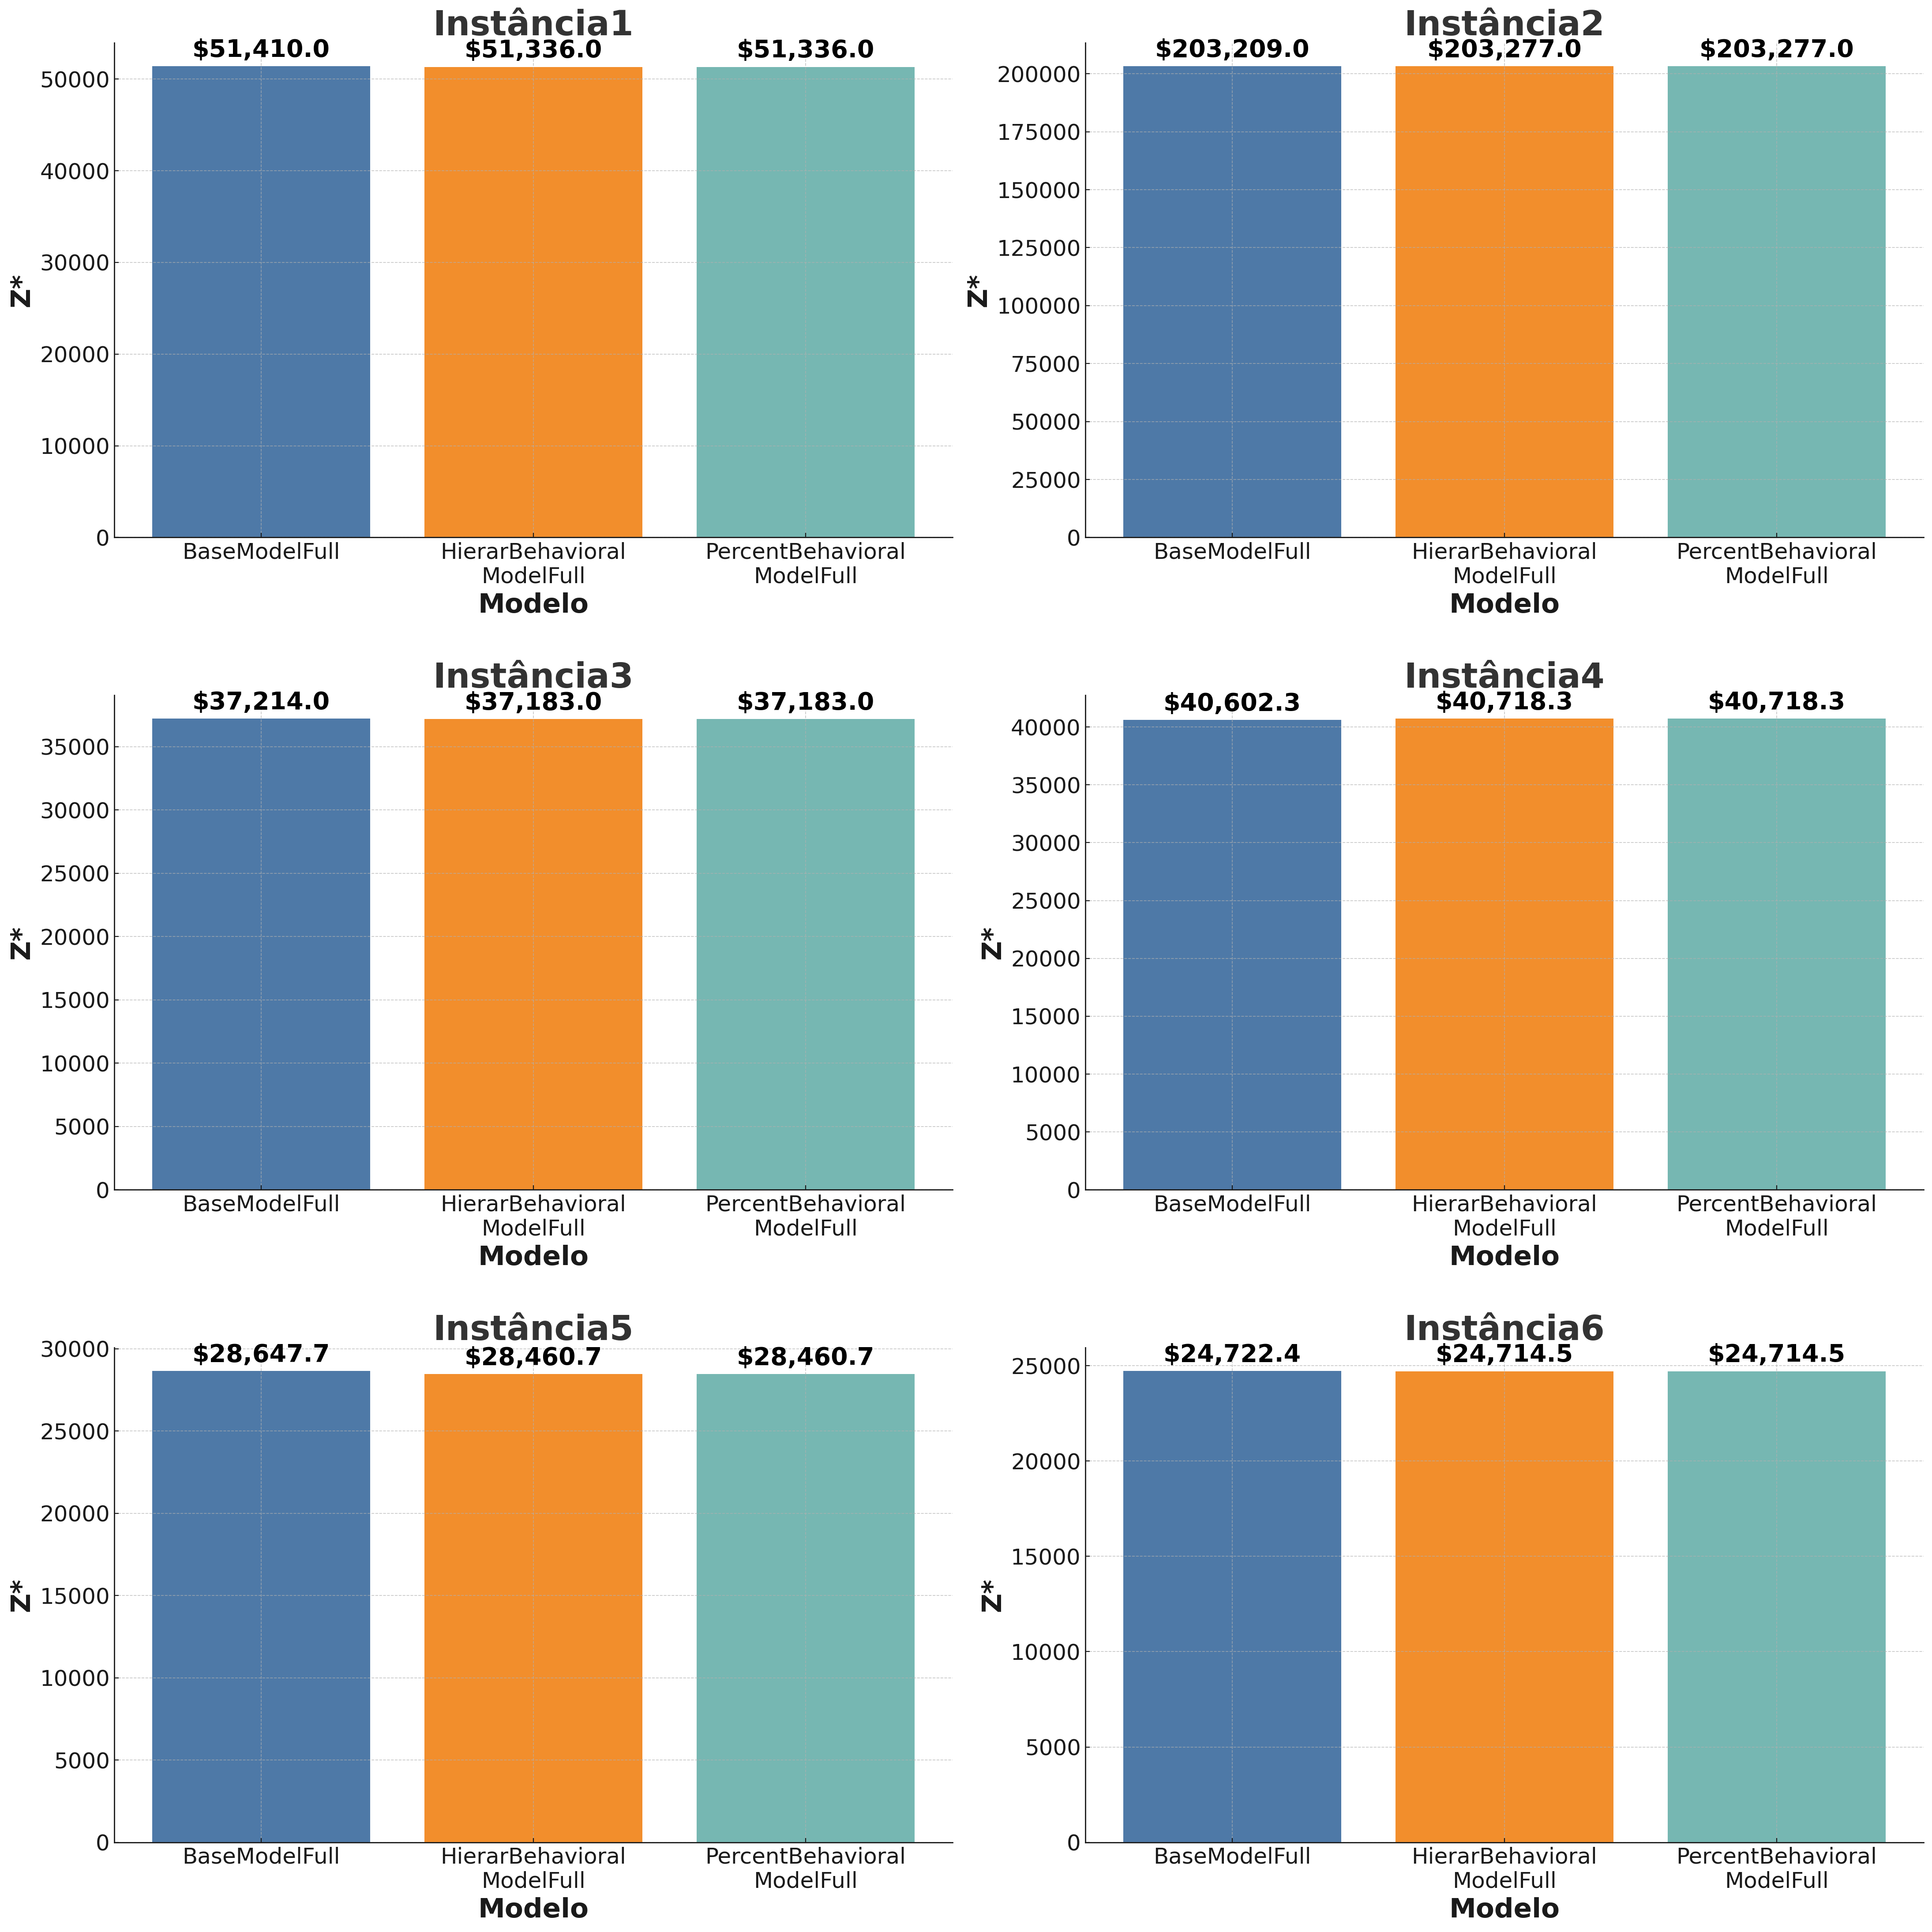
\includegraphics[scale=0.28]{img/compFull1.png}
		\caption{Comparação Modelos Full primeira parte}
		% Fonte:~\cite{khaksar2013genetic}}
		\label{fig: compfull1}
	\end{center}
\end{figure}

\begin{figure}[!ht]
	\begin{center}
		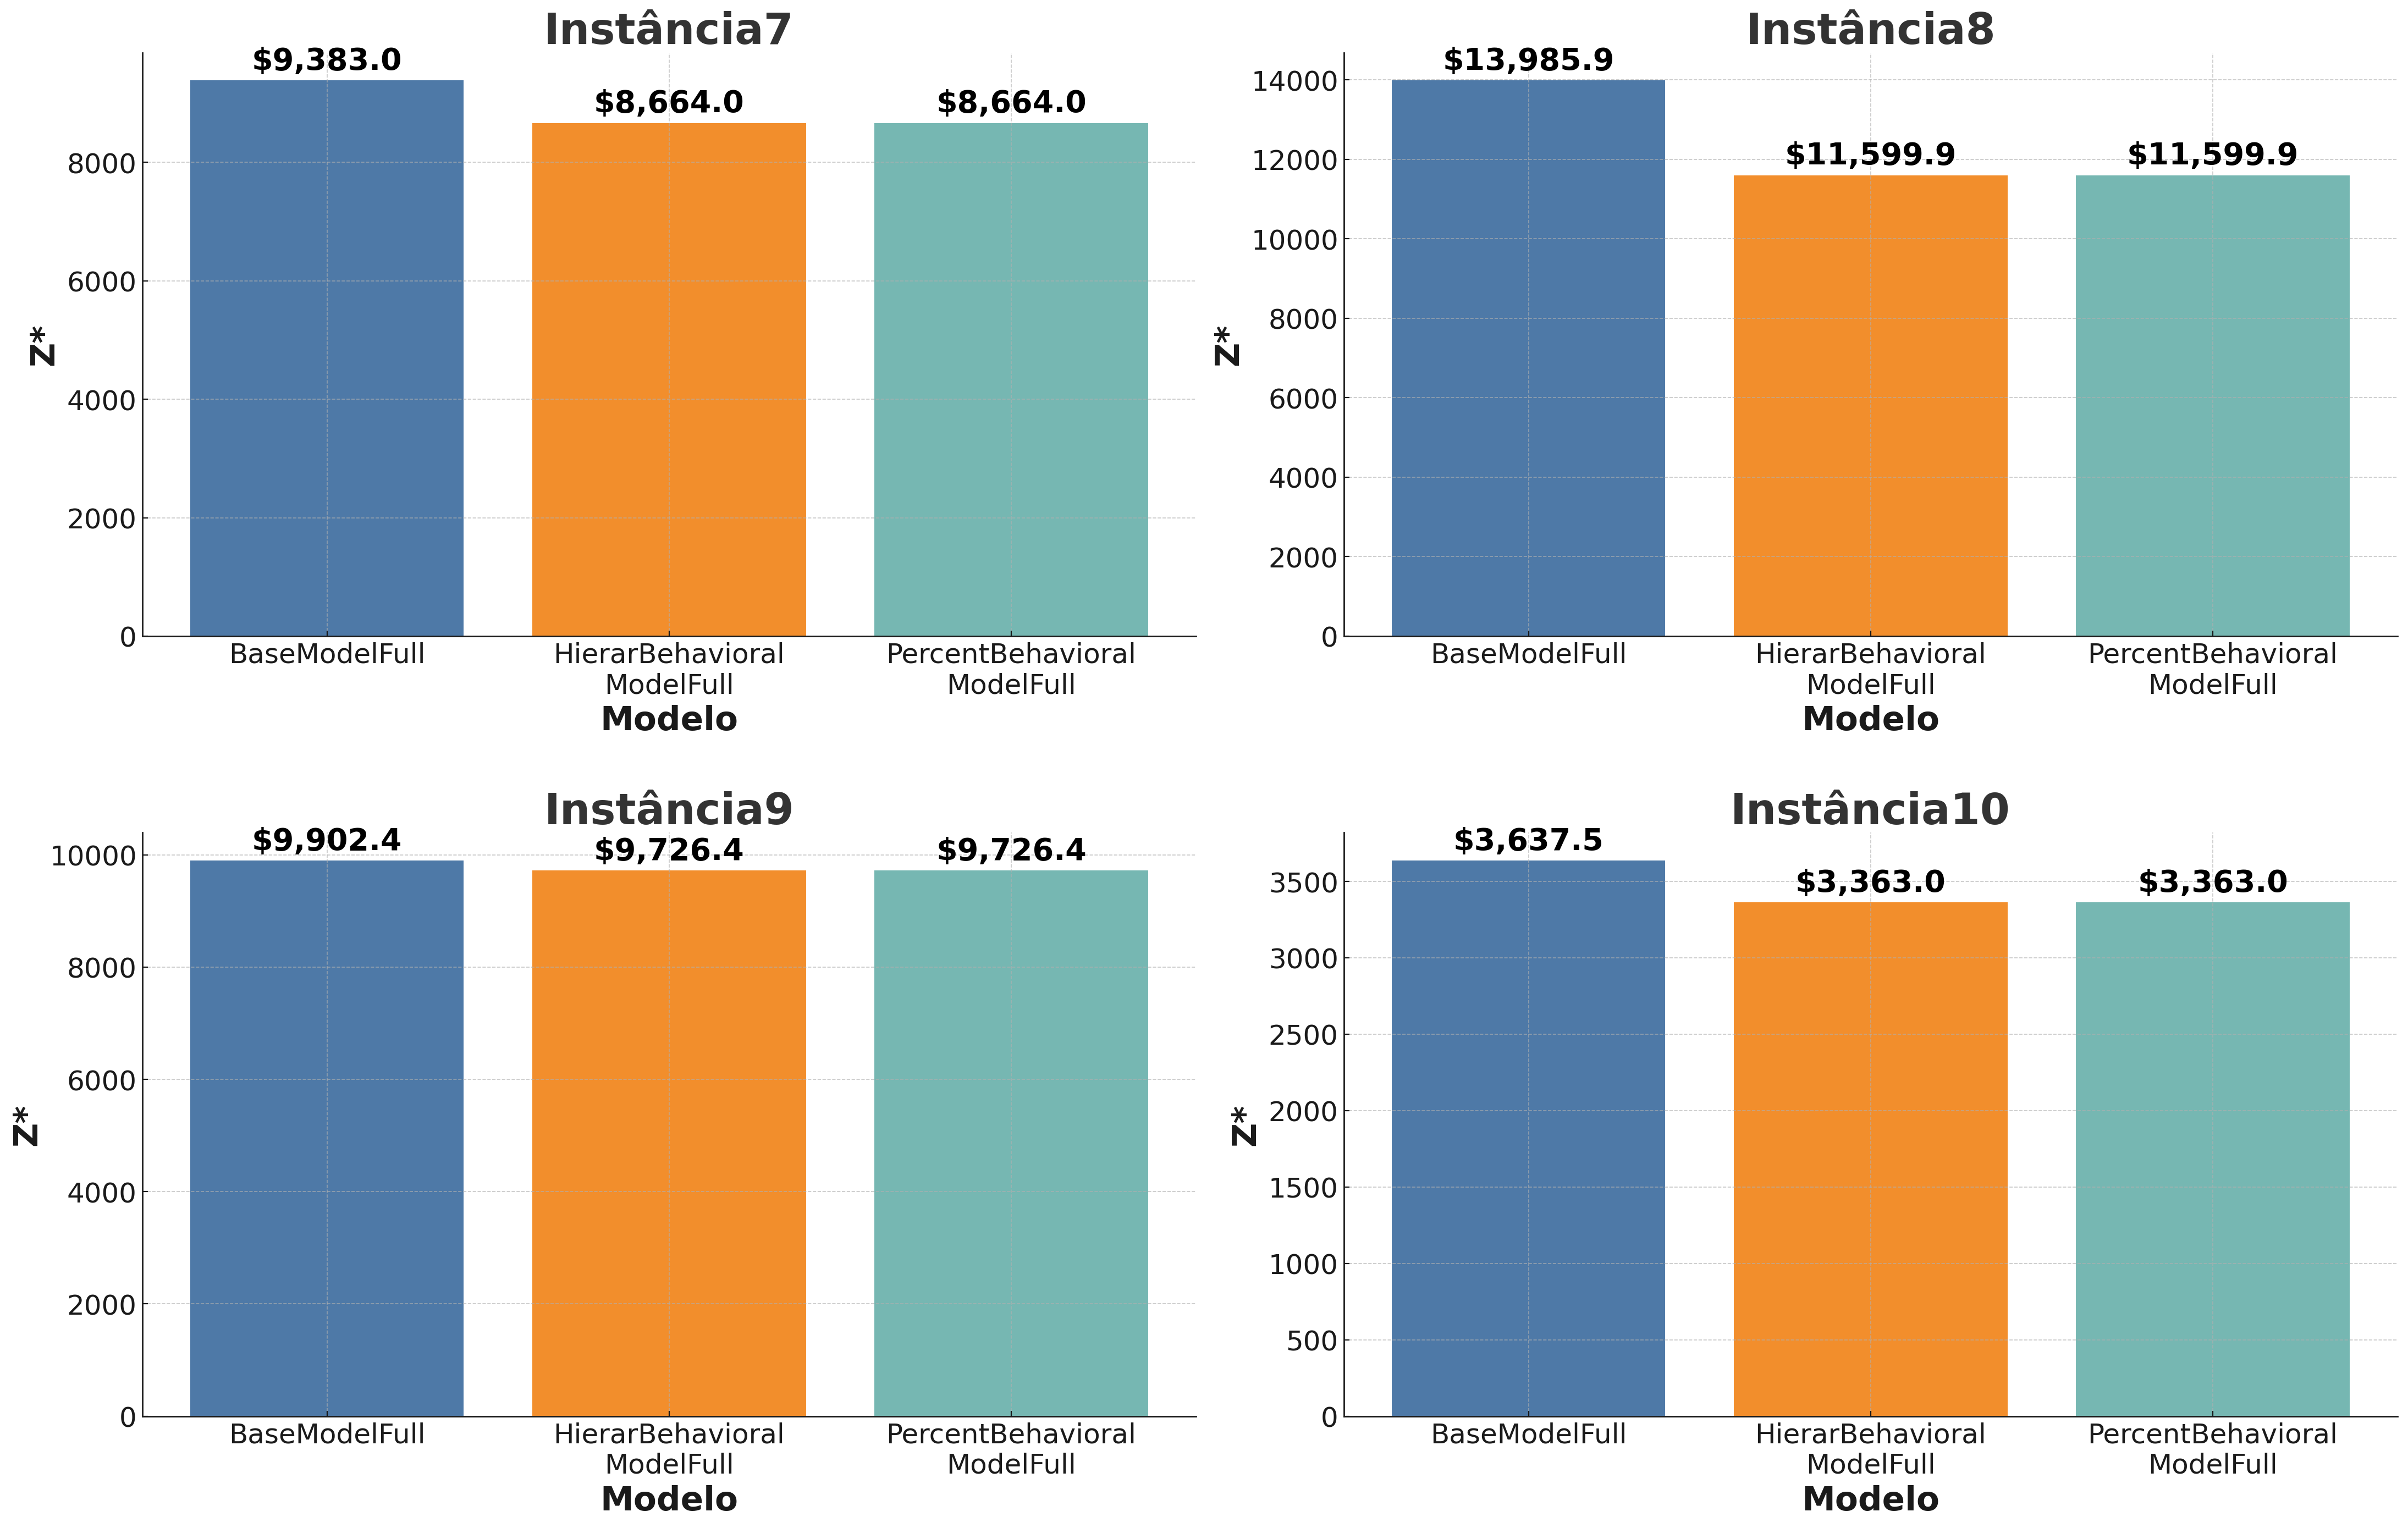
\includegraphics[scale=0.28]{img/compFull2.png}
		\caption{Comparação Modelos Full segunda parte}
		% Fonte:~\cite{khaksar2013genetic}}
		\label{fig: compfull2}
	\end{center}
\end{figure}


Dentro dos resultados observados, diversos comportamentos interessantes foram identificados:

\begin{enumerate}
    \item Tempo de solução:
    O tempo necessário para resolver cada modelo em todas as instâncias foi relativamente baixo. Por exemplo:
    \begin{itemize}
    \item Para as instâncias grandes, os tempos variaram entre 0,04 e 0,12 segundos;
    \item Para as instâncias médias, entre 0,02 e 0,08 segundos;
    \item Para as instâncias pequenas, entre 0,00 e 0,07 segundos.
    \end{itemize}

    \item Exploração de nós:
    Os modelos sempre alcançaram a solução ou soluções ótimas explorando, no máximo, um único nó. Isso demonstra que, na maioria dos casos, a solução ótima coincide com a relaxação linear. Quando isso não ocorre, a diferença máxima relativa é de apenas 0,01\%.
    
    \item Modelos com demanda independente:
    \begin{itemize}
        \item Os modelos BaseModel e BaseModelFulfillments produziram exatamente os mesmos resultados em todas as instâncias analisadas;
        \item O modelo BaseModelSkiplagging, em comparação com o BaseModelFulfillments, apresentou uma redução relativa entre 21,25\% e 56,90\% em todas as instâncias, exceto na instância instância2, onde a redução foi de apenas 3,57\%;
        \item O modelo BaseModelFull mostrou uma redução ainda maior, variando entre 21,25\% e 72,24\%, em comparação com o BaseModelSkiplagging, novamente com exceção da instância instância2, onde a redução foi de 3,57\%.
    \end{itemize}

    \item Modelos com demanda comportamental ajustada por proporções:
    \begin{itemize}
        \item Não foram observadas diferenças entre os modelos BaseModel e BaseModelFulfillments;
        \item Ao contrário do comportamento no modelo independente, o modelo PercentBehavioralModelFulfillments apresentou um aumento relativo entre 0,33\% e 8,6\% nas soluções obtidas, em comparação com o modelo HierarBehavioralModel, exceto nas instâncias instância7, instância8 e instância10, onde o HierarBehavioralModel foi inviável. Acredita-se que essa inviabilidade se deva a alguma inconsistência gerada durante o ajuste da demanda, mas a causa exata ainda não foi determinada;
        \item O modelo PercentBehavioralModelFull mostrou uma redução relativa entre 33\% e 70\%, em comparação com o modelo PercentBehavioralModelSkiplagging.
    \end{itemize}

    \item Modelos com demanda comportamental ajustada por hierarquia:
    \begin{itemize}
        \item Os modelos HierarBehavioralModel e HierarBehavioralModelFulfillments apresentaram os mesmos resultados em todas as instâncias, exceto nas instâncias instância3 e instância6, onde ocorreram reduções de 0,06\% e 0,01\%, respectivamente;
        \item O modelo HierarBehavioralModelSkiplagging apresentou reduções entre 21,8\% e 56,9\%, exceto na instância instância1, onde a redução foi de apenas 3,57\%;
        \item O modelo HierarBehavioralModelFull registrou reduções consideráveis em relação ao modelo HierarBehavioralModelSkiplagging, variando entre 33\% e 74\%.
    \end{itemize}

    \item Análise dos modelos Full (BaseModelFull, HierarBehavioralModelFull, PercentBehavioralModelFull):
    \begin{itemize}
        \item Considerando apenas os modelos Full, ou seja, aqueles que incluem todos os conjuntos de restrições, os modelos comportamentais obtiveram exatamente os mesmos resultados para a função objetivo em cada instância. No entanto, como algumas instâncias possuem múltiplas soluções ótimas, os valores das variáveis de decisão podem diferir, mesmo que os valores da função objetivo sejam iguais;
        \item Além disso, a diferença entre os modelos comportamentais e o modelo independente foi de, no máximo, 2\%, exceto nas instâncias instância7 e instância8, onde as variações foram de 7,7\% e 16,1\%, respectivamente.
    \end{itemize}

\end{enumerate}


Esse detalhamento evidencia o comportamento dos modelos e suas respectivas eficiências em diferentes cenários e ajustes.